\documentclass[aspectratio=169]{beamer}

\usetheme{Madrid}
\usecolortheme{default}
\setbeamertemplate{navigation symbols}{}

\usepackage{graphicx}
\usepackage{booktabs}
\usepackage{amsmath}

\title[Image Dehazing with AOD-Net]{Image Dehazing using AOD-Net\\with Residual Learning and Skip Connections}
\author{Ritwick Ranjan}
\institute{Department of Computer Science \\ Your Institute Name}
\date{April 2026}

\begin{document}

\begin{frame}
  \titlepage
\end{frame}

\begin{frame}{Problem Statement}
  \begin{itemize}
    \item Atmospheric haze reduces contrast, weakens edges, and makes downstream vision tasks less reliable.
    \item Classical dehazing methods often depend on hand-crafted priors and may fail on diverse real scenes.
    \item This project studies whether a lightweight CNN, AOD-Net, can be adapted into a simple academic pipeline with two enhancements:
    \begin{itemize}
      \item residual learning
      \item skip connections
    \end{itemize}
    \item Goal: build a modular notebook and an interactive web demo that accept a hazy image and return a dehazed result.
  \end{itemize}
\end{frame}

\begin{frame}{Objectives}
  \begin{itemize}
    \item Reproduce the core AOD-Net logic from the reference PyTorch repository.
    \item Train and compare three lightweight variants on the RESIDE-6K dataset.
    \item Evaluate using MSE loss and PSNR.
    \item Present qualitative and quantitative evidence in a beginner-friendly workflow.
    \item Extend the project into a web-based interface for real-time image upload and dehazing.
  \end{itemize}
\end{frame}

\begin{frame}{Baseline AOD-Net}
  \begin{itemize}
    \item AOD-Net is a compact convolutional dehazing model proposed to estimate a clean image directly from hazy input.
    \item The model uses stacked convolutions to predict a feature map \(k(x)\) and reconstruct the output with a haze-aware formulation:
  \end{itemize}
  \[
    J(x) = k(x)\cdot I(x) - k(x) + b
  \]
  \begin{itemize}
    \item In this project, the original architecture was kept lightweight for easy training and presentation.
    \item The baseline serves as the reference point for the enhanced variants.
  \end{itemize}
\end{frame}

\begin{frame}{Enhanced Variants}
  \begin{block}{Residual Variant}
    The network predicts a haze residual and subtracts it from the input:
    \[
      \hat{J}(x) = I(x) - R(x)
    \]
  \end{block}

  \begin{block}{Skip-Connection Variant}
    A learnable skip-fusion path combines the network prediction with the input image to preserve structural details:
    \[
      \hat{J}(x) = F(I(x)) + \alpha \odot I(x)
    \]
  \end{block}

  \begin{itemize}
    \item Residual learning simplifies the target signal.
    \item Skip fusion helps retain edges and local textures.
  \end{itemize}
\end{frame}

\begin{frame}{Dataset and Training Setup}
  \begin{itemize}
    \item Dataset: Kaggle RESIDE-6K image pairs.
    \item Preprocessing: RGB conversion and resize to \(256 \times 256\).
    \item Training subset used for the lightweight demo: 600 paired images.
    \item Split: 80\% training and 20\% validation.
    \item Loss: Mean Squared Error.
    \item Optimizer: Adam, learning rate \(= 10^{-3}\), batch size \(= 8\), epochs \(= 6\).
    \item Platform: PyTorch CPU training pipeline aligned with the notebook and web app.
  \end{itemize}
\end{frame}

\begin{frame}{Quantitative Results}
  \begin{table}
    \centering
    \small
    \begin{tabular}{lccc}
      \toprule
      Model & Best Epoch & Val. Loss & Val. PSNR (dB) \\
      \midrule
      Baseline AOD-Net & 4 & 0.0163 & 19.50 \\
      Residual AOD-Net & 6 & 0.0177 & 18.89 \\
      Skip AOD-Net & 4 & 0.0163 & 19.65 \\
      \bottomrule
    \end{tabular}
  \end{table}

  \vspace{0.5em}
  \begin{itemize}
    \item The skip-connection model achieved the strongest saved-checkpoint PSNR.
    \item The residual model remained stable but did not surpass the baseline under the current training budget.
    \item The results show that lightweight architectural changes can affect restoration quality meaningfully.
  \end{itemize}
\end{frame}

\begin{frame}{Training Curves}
  \begin{columns}[T]
    \column{0.5\textwidth}
    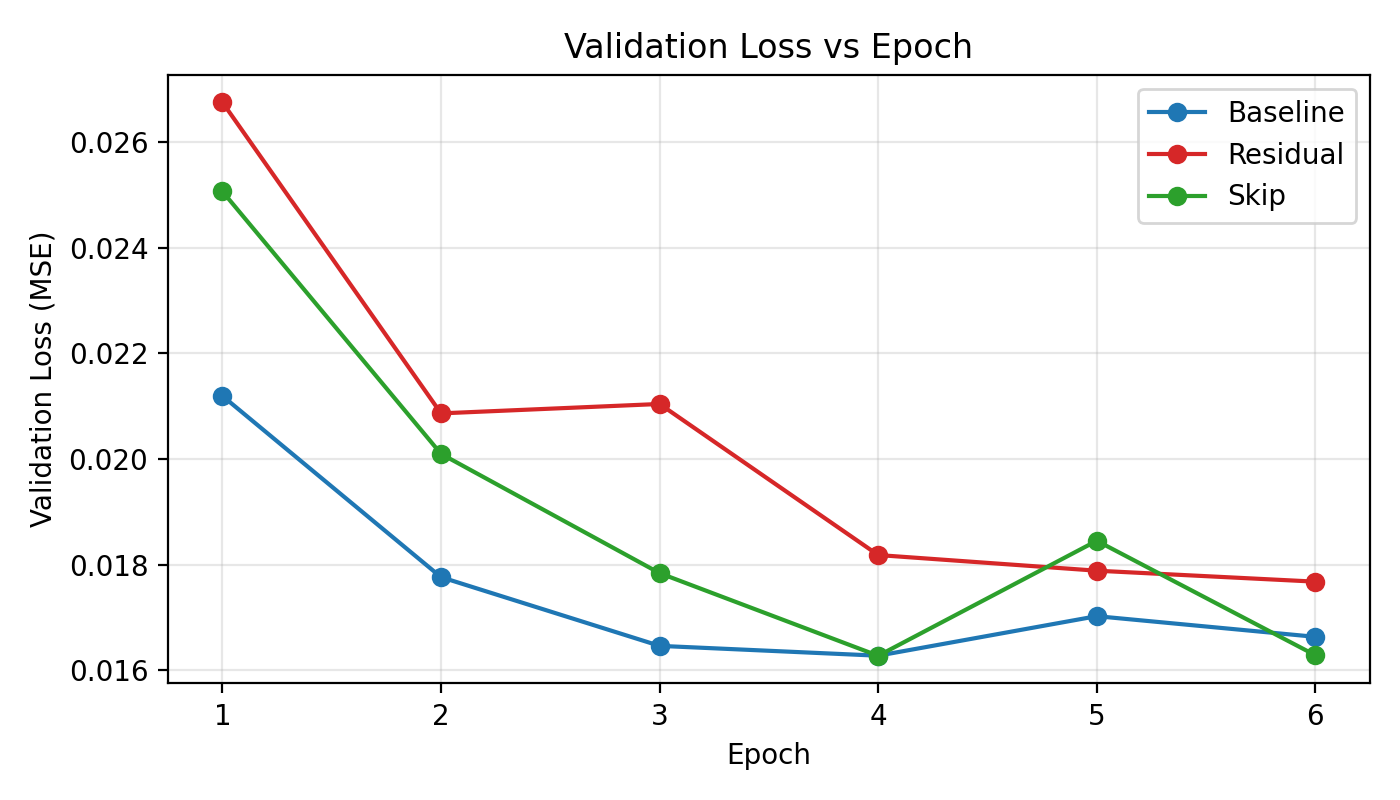
\includegraphics[width=\linewidth]{../assets/loss_curves.png}

    \column{0.5\textwidth}
    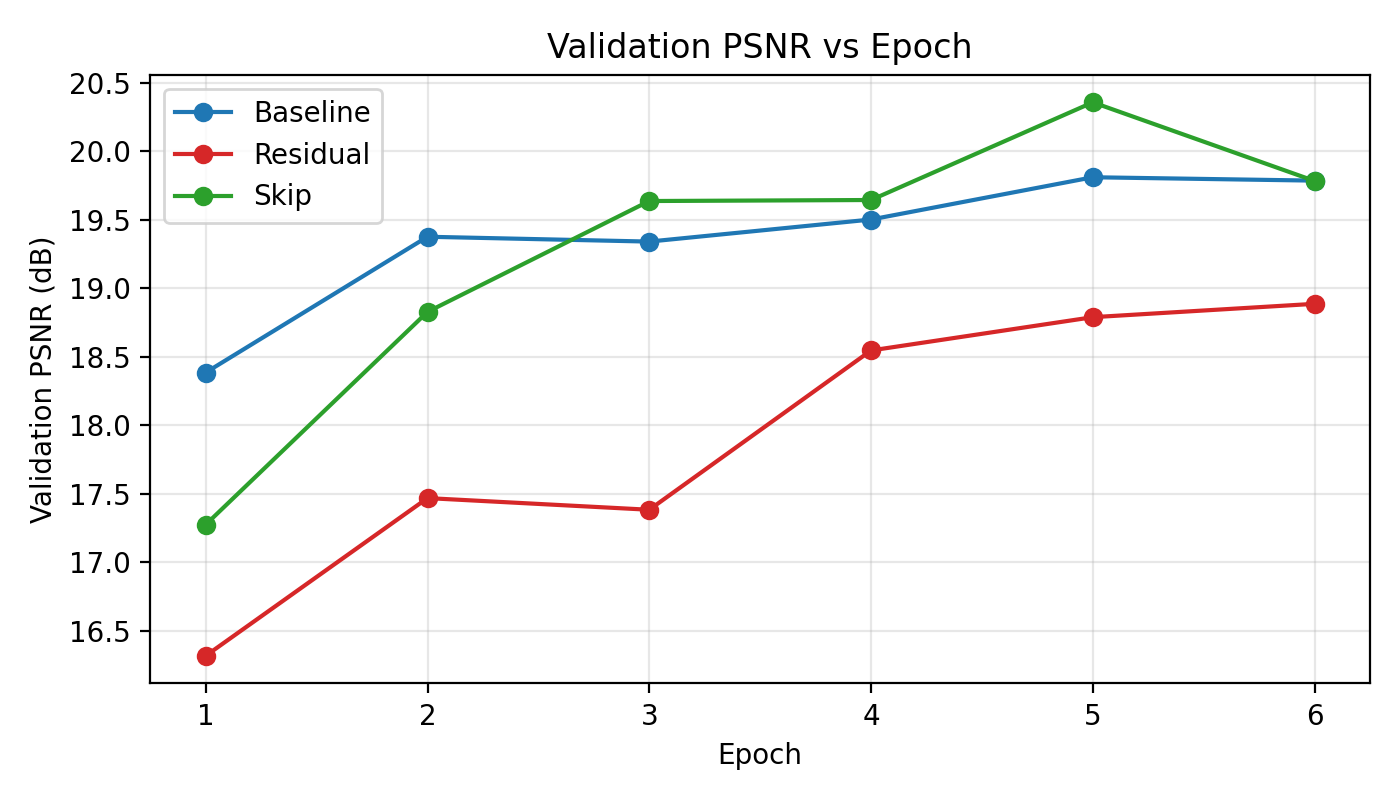
\includegraphics[width=\linewidth]{../assets/psnr_curves.png}
  \end{columns}

  \vspace{0.5em}
  \begin{itemize}
    \item Validation loss decreases rapidly in the first few epochs.
    \item PSNR trends show the skip variant peaking slightly above the baseline.
  \end{itemize}
\end{frame}

\begin{frame}{Qualitative Comparison}
  \centering
  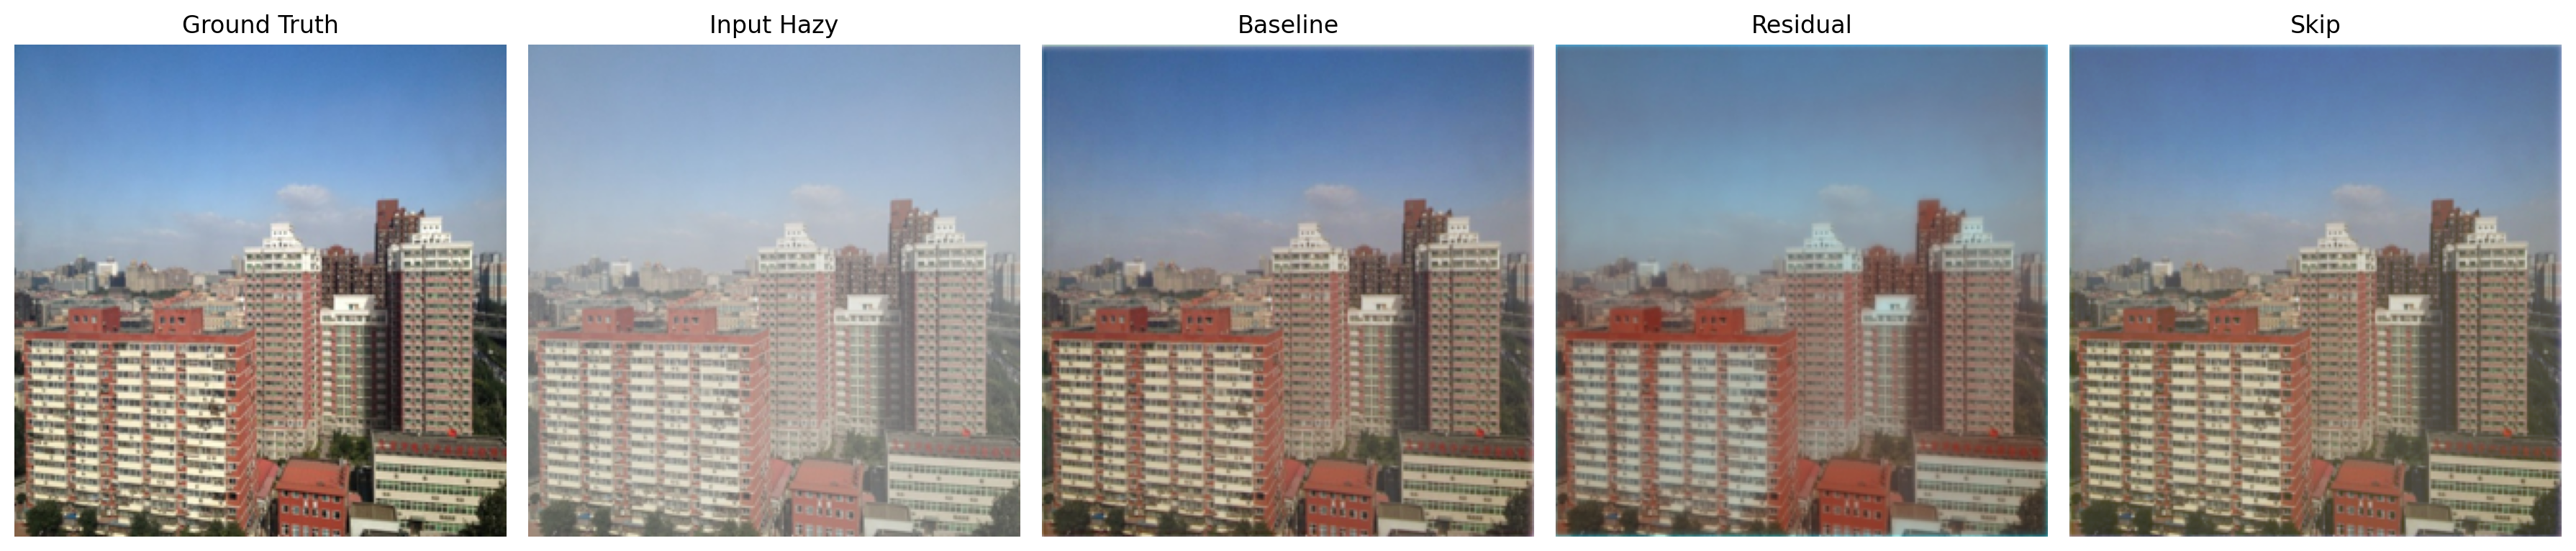
\includegraphics[width=\linewidth]{../assets/comparison_panel.png}

  \vspace{0.4em}
  \begin{itemize}
    \item All models improve visibility compared with the hazy input.
    \item The skip-based result preserves scene structure more effectively in this sample.
  \end{itemize}
\end{frame}

\begin{frame}{Interactive Web Demo}
  \begin{itemize}
    \item A Gradio-based interface was added on top of the trained checkpoints.
    \item Users can upload a hazy image, choose a model variant, and instantly view the dehazed output.
    \item The demo reuses the same trained models and preprocessing pipeline as the notebook.
  \end{itemize}

  \begin{block}{Workflow}
    Upload image \(\rightarrow\) select model \(\rightarrow\) run inference \(\rightarrow\) save or inspect dehazed output
  \end{block}

  \begin{itemize}
    \item This makes the project more presentation-friendly and easier to explain live.
  \end{itemize}
\end{frame}

\begin{frame}{Key Takeaways}
  \begin{itemize}
    \item AOD-Net provides a compact and interpretable baseline for image dehazing.
    \item Residual learning offers a simple reformulation of the dehazing objective.
    \item Skip connections improved saved-checkpoint PSNR in the current experiments.
    \item The project now exists as:
    \begin{itemize}
      \item a step-by-step notebook
      \item trained checkpoints
      \item an interactive web application
      \item a slide deck and IEEE-style paper
    \end{itemize}
  \end{itemize}
\end{frame}

\begin{frame}{Future Scope}
  \begin{itemize}
    \item Train on the full RESIDE split rather than a lightweight subset.
    \item Add SSIM and perceptual metrics for stronger evaluation.
    \item Improve the residual branch with deeper supervision and longer training.
    \item Extend the web app with drag-and-drop comparison and downloadable reports.
  \end{itemize}
\end{frame}

\begin{frame}
  \centering
  \Huge Thank You
\end{frame}

\end{document}
